\chapter{La diffraction}
\begin{wrapfigure}[8]{r}{2cm}
\vspace{-6mm}
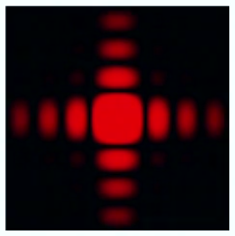
\includegraphics[scale=0.30]{ch2/image4.png}
\captionof{figure}{ }
\end{wrapfigure}
Un faisceau laser se propageant à tendance à s'élargir et se déformer : il s'agit du 
phénomène de diffraction. Ce phénomène est bien précis et peut être décrit mathématiquement. 
Il dépend notamment de la forme du laser. En faisant passer un laser par une section carrée, 
on sera amener à observer des distributions d'intensités particulières.

\section{Équations de Maxwell et transformée de Fourier}
La linéarité des équations de Maxwell permet un traitement efficace par les transformées 
de Fourier. Voici les fameuses équations dans le vide
\begin{equation}
\left\{\begin{array}{llll}
\rot \vec{E} &= -\dfrac{\partial \vec{B}}{\partial t},\qquad &\div \vec{E} &= 0\\
\rot \vec{B} &= \epsilon_0\mu_0\dfrac{\partial \vec{E}}{\partial t},\qquad &\div \vec{B} &= 0
\end{array}\right.
\end{equation}
Sachant que $\rot [\rot \vec{E}] = \grad[\div \vec{E}] - \Delta\vec{E}$ où $\div \vec{E}=0$ dans 
le vide on retrouve l'équation d'onde électromagnétique
\begin{equation}
\Delta \vec{E} = \mu_0\epsilon_0\dfrac{\partial^2\vec{E}}{\partial t^2}\quad \text{où } \Delta 
\vec{E} = \Delta E_x\vec{1_x}+\Delta E_y\vec{1_y}+\Delta E_z\vec{1_z}
\end{equation}
On ne considérera ici que la composante en $x$ du champ
\begin{equation}
\Delta E_x = \mu_0\epsilon_0\dfrac{\partial^2E_x}{\partial t^2}
\end{equation}
On remplacera souvent $E_x,E_y$ ou $E_z$ par $E$ mais il faut garder à l'idée qu'il ne s'agit 
qu'une seule des composantes du champ. L'équation d'onde scalaire s'écrit
\begin{equation}
\dfrac{\partial E}{\partial x^2}+\dfrac{\partial E}{\partial y^2}+\dfrac{\partial E}{\partial z^2} 
= \mu_0\epsilon_0\dfrac{\partial^2E}{\partial t^2}
\end{equation}
Cette équation est \textit{linéaire}, $E$ n'apparaissant qu'à la première puissance. Si $E_1$ et 
$E_2$ sont solution, une combili de ces deux solutions est également solution. On va profiter 
de cette linéarité pour exprimer la solution de cette équation comme une somme d'onde harmonique, 
d'où l'utilité des transformée de Fourier. Le champ électrique se verra décomposé en une somme 
de \textit{fonctions harmonique}\footnote{Écrit ci-dessous dans le domaine des phaseurs.} :
\begin{equation}
E(x,y,z,t) = \iiiint_{-\infty}^\infty \tilde{E}(k_x,k_y,k_z,\omega)e^{ik_xx}e^{ik_yy}e^{ik_zz}
e^{-i\omega t}\ dk_xdk_ydk_zd\omega
\end{equation}
Si le facteur harmonique $e^{ik_xx}e^{ik_yy}e^{ik_zz}e^{-i\omega t}$  est solution des équations 
de Maxwell $\forall k_i,\omega$, alors $E$ sera solution. La résolution de ces équations ne sont 
pas aisées. Pour le faire de façon analytique, on travaillera avec la décomposition. Vérifions 
que ces fonctions harmoniques sont bien solution
\begin{equation}
\dfrac{\partial^2 e^{ik_xx}e^{ik_yy}e^{ik_zz}e^{-i\omega t}}{\partial x^2} = -k_x^2 e^{ik_xx}e^{ik_yy}
e^{ik_zz}e^{-i\omega t}
\end{equation}
En faisant de même pour les deux autres dérivées partielles pour obtenir
\begin{equation}
(-k_x^2-k_y^2-k_z^2)e^{ik_xx}e^{ik_yy}e^{ik_zz}e^{-i\omega t} = -\mu_0\epsilon_0\omega^2 
e^{ik_xx}e^{ik_yy}e^{ik_zz}e^{-i\omega t}
\end{equation}
C'est-à-dire
\begin{equation}
k_x^2+k_y^2+k_z^2 = \mu_0\epsilon_0\omega^2
\end{equation}
Il s'agit d'une \textbf{contrainte} sur les modes de Fourier. On peut voir l'expression de $E$ 
comme une transformée de Fourier où $\tilde{E}$ est le spectre de Fourier généralisé à 4 
dimensions. En terme de transformée de Fourier, on peut dire qu'il s'agit d'une contrainte 
sur les \textit{modes de Fourier} (les quatre facteurs exponentiels), soit une \textbf{relation 
de dispersion généralisée}. Si les modes satisfont cette contrainte, $E$ sera solution.\\

\begin{wrapfigure}[9]{r}{3cm}
%\vspace{-6mm}
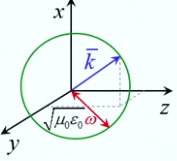
\includegraphics[scale=0.45]{ch2/image5.png}
\captionof{figure}{ }
\end{wrapfigure}
Intéressons-nous aux aspects physiques sous-jacent à cette décomposition de Fourier du champ 
électrique. Commençons par la ré-écriture suivante en supposant que les $k_i$ sont les 
composantes d'un vecteur
\begin{equation}
\tilde{E}(k_x,k_y,k_z,\omega)e^{ik_xx}e^{ik_yy}e^{ik_zz}e^{-i\omega t} = \tilde{E}(\vec{k},
\omega)e^{i\vec{k}.\vec{r}}e^{-i\omega t}
\end{equation}
\danger $\vec{r}$ est le vecteur position, il désigne le point de l'espace considéré. On peut 
ainsi exprimer la condition pour laquelle le mode de Fourier satisfait les équations de Maxwell  :
\begin{equation}
|k|^2 = k^2 = \mu_0\epsilon_0\omega^2
\end{equation}

\begin{wrapfigure}[9]{l}{3cm}
\vspace{-6mm}
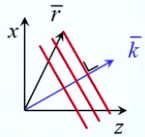
\includegraphics[scale=0.45]{ch2/image6.png}
\captionof{figure}{ }
\end{wrapfigure}
Cela signifie que le vecteur d'onde est tendu d'être sur une sphère de rayon $k=
\sqrt{\mu_0\epsilon_0}\omega$. Figeons le temps et cherchons le lieux des points de phase 
constante. Pour avoir une phase constante, $\vec{k}.\vec{r}$ doit être constant : tous les 
points qui ont la même projection auront la même phase, il s'agit d'une \textit{onde plane}.
Ci-contre, la représentation des fronts d'ondes. Analysons cela de façon analytique
\begin{equation}
\varphi = \vec{k}.\vec{r} = \text{cste}\quad \Rightarrow k_xx+k_yy+k_zz = \text{ cste}
\end{equation}
Il s'agit de l’équation d'un plan perpendiculaire au vecteur d'onde. Les modes de Fourier 
réprésentent bien une onde plane dont la direction $\vec{k}/k$. On peut toujours considérer 
$\vec{k}/k = \vec{1_z} \rightarrow \vec{k}= k\vec{1_z}$ de sorte à écrire
\begin{equation}
E = \tilde{E}e^{ikz}e^{-i\omega t}
\end{equation}
Ceci montre que lorsque $z$ est fixé, le champ ne varie pas en $x$. Si l'on considère la 
partie réelle de ceci, on retrouve $\tilde{E}\cos(kz-\omega t)$ ce qui est bien l'équation 
d'une onde plane.\\

Que se passe-t-il si on libère le temps? Intéressons-nous d'abord à la périodicité en 
$z : \lambda = 2\pi/k$ ce qui correspond à l'espacement des fronts d'ondes. Considérons 
une phase constante
\begin{equation}
\text{Front d'onde : } \varphi = \text{ cste} \Rightarrow  kz-\omega t = \text{ cste} \qquad 
\Longleftrightarrow z = \dfrac{\omega}{k}t+\dfrac{\text{cste}}{k}
\end{equation}
Pour garder la constante, quand le temps augmente $z$ doit également augmenter. On obtient 
ici la \textit{vitesse de phase} $\omega/k = v_\phi$ où $k = \sqrt{\mu_0\epsilon_0}\omega$. 
Cette dernière condition est obligatoire pour avoir quelque chose de physique vérifiant 
les équations de Maxwell. Par substitution
\begin{equation}
v_\varphi = \dfrac{1}{\sqrt{\mu_0\epsilon_0}} \equiv c
\end{equation}
On en tire que $k=\omega/c$.\\

\underline{Remarque}. Considérons un champ scalaire solution des équations d'ondes 
\begin{equation}
\vec{E} = (A_x\vec{1_x}+A_y\vec{1_y}+A_z\vec{1_z})e^{ikz}e^{ikz}e^{-i\omega t}
\end{equation}
où les amplitudes $A_i$ ne sont pas nécessairement connues. Nous allons voir qu'il y a 
une contrainte sur ces amplitudes. Appliquons la divergence nulle du champ électrique 
dans le vide
\begin{equation}
\div \vec{E} = 0 \quad \Longrightarrow\quad \dfrac{\partial E_x}{\partial x}+
\dfrac{\partial E_y}{\partial y} + \dfrac{\partial E_z}{\partial z} = 0
\end{equation}

\begin{wrapfigure}[6]{l}{3cm}
\vspace{-16mm}
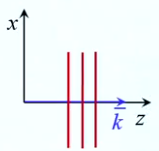
\includegraphics[scale=0.45]{ch2/image7.png}
\captionof{figure}{ }
\end{wrapfigure}
Or, il n'y a pas de dépendance en $x$ et $y$ comme le montre le schéma ci-contre. Avoir 
une composante selon $y$, ici $A_y$ n'implique pas une dépendance en $y$! Dès lors, 
seule la dérivée par rapport à $z$ est non-nulle. On en tire
\begin{equation}
iA_zke^{ikz}e^{-i\omega t} = 0\qquad \forall z,t
\end{equation}
Il en résulte que $A_z = 0$. Conclusion : le champ électrique est toujours transverse à 
l'axe $z$ pour une onde se déplaçant sur ce même axe.\\

Revenons à la description mathématique de la SG des EDP de Maxwell. Rappelons la \textbf{contrainte 
sur les modes de Fourier} 
\begin{equation}
k = \dfrac{\omega}{c}
\end{equation}
Le vecteur d'onde doit obligatoirement se balader sur une sphère :
\begin{equation}
k_x^2+k_y^2+k_z^2 = k^2 = \dfrac{\omega^2}{c}
\end{equation}
Rentrons cette contrainte dans l'expression de $E$. Or, nous n'avons que trois dimension : on 
fait le choix d'exprimer $k_z$ en fonction de la contrainte :
\begin{equation}
k_z = \sqrt{k^-k_x^2-k_y^2}
\end{equation}
Si $k_z$ satisfait cette relation, c'est gagné. Pour être solution, il faut que le spectre ai 
la forme particulière définie ci-dessous, qui ne dépend plus de $k_z$ la variable ayant été 
"sacrifiée" :
\begin{equation}
\tilde{E}(k_x,k_y,k_z,\omega) = \tilde{E}(k_x,k_y,\omega)\delta\left(k_z-\sqrt{k^-k_x^2-k_y^2}\right)
\end{equation}
où l'on introduit le delta de Dirac : si le spectre est limité à des spectres de cette forme là, 
d'office ce sera solution des équations de Maxwell\footnote{C'est une façon mathématique d'imposer 
la valeur de $k_z$.}. En substituant dans mon équation $\iiiint$, une des intégrales sera simplifiée 
par le delta de Dirac.
\begin{equation}
E(x,y,z,t) = \iiint_{-\infty}^\infty \tilde{E}(k_x,k_y,\omega) e^{ik_xx}e^{ik_yy}e^{i 
\sqrt{k^-k_x^2-k_y^2} z}e^{-i\omega t}\ dk_xdk_yd\omega
\end{equation}
Ce qui n'est rien d'autre que la solution générale des équations de Maxwell. Nous allons nous limiter 
à des ondes monochromatiques, c'est à dire pour un seul $\omega_0$. On se limite ainsi à un spectre 
spatial pour une fréquence donnée
\begin{equation}
\tilde{E}(k_x,k_y,\omega) = A(k_x,k_y)\delta(\omega-\omega_0)
\end{equation}
Notre intégrale triple devient
\begin{equation}
E(x,y,z,t) = \iint_{-\infty}^\infty A(k_x,k_y) e^{ik_xx}e^{ik_yy}e^{i 
\sqrt{k^-k_x^2-k_y^2} z}\ dk_xdk_ye^{-i\omega_0 t}
\end{equation}
où $\omega$ n'apparaît plus : il est caché dans la définition de $k$. On considère ici des ondes 
monochromatiques, on va dès lors s'affranchir du caractère temporel qui ne nous intéresse pas ici. 
Soit 
\begin{equation}
E(x,y,z,t) = a(x,y,z)e^{-i\omega_0t}
\end{equation}
où $a$ est l'amplitude indépendante du temps. On a donc
\begin{equation}
a(x,y,z) = \iint_{-\infty}^\infty A(k_x,k_y) e^{ik_xx}e^{ik_yy}e^{i 
\sqrt{k^-k_x^2-k_y^2} z}\ dk_xdk_y
\end{equation}
où $k^2 = \omega_0^2/c^2$. Ceci est à coup sur une solution des équations de Maxwell. Allégeons 
les notations : $k_x=\rho, k_y=\sigma, k_z=\beta=\sqrt{k^2-\rho^2-\sigma^2}$ pour avoir
\begin{equation}
a(x,y,z) = \iint_{-\infty}^\infty A(\rho,\sigma)e^{i\rho x}e^{i\sigma y} e^{i\sqrt{k^2-\rho^2-
\sigma^2}z}\ d\rho d\sigma
\end{equation}
Il s'agit d'une intégrale de Fourier, une combinaison linéaire d'onde plane qui ont certaines 
amplitudes qui représentent le spectre du champ. Il s'agit de l'expression d'une \textit{solution 
générale des équations de Maxwell pour une onde monochromatique}, le point de départ de la 
théorie de diffraction.

















































